% !TEX root = hazelnut-dynamics.tex

\begin{figure}[t]

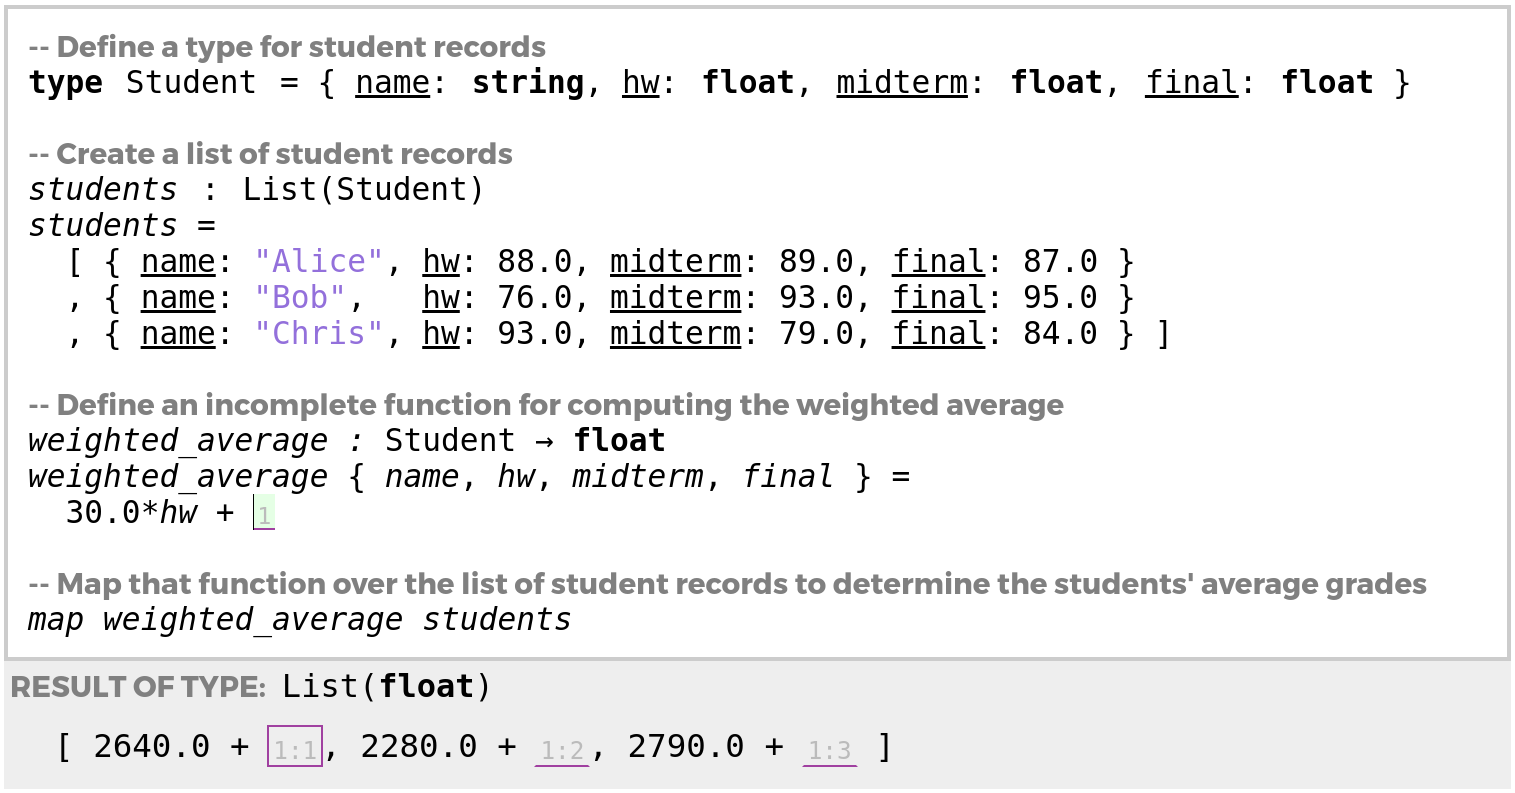
\includegraphics[width=1.01\textwidth,interpolate=false]{images/grades-cell-mockup.png}

% %% TODO once the code above is removed, scale up the screenshots
% 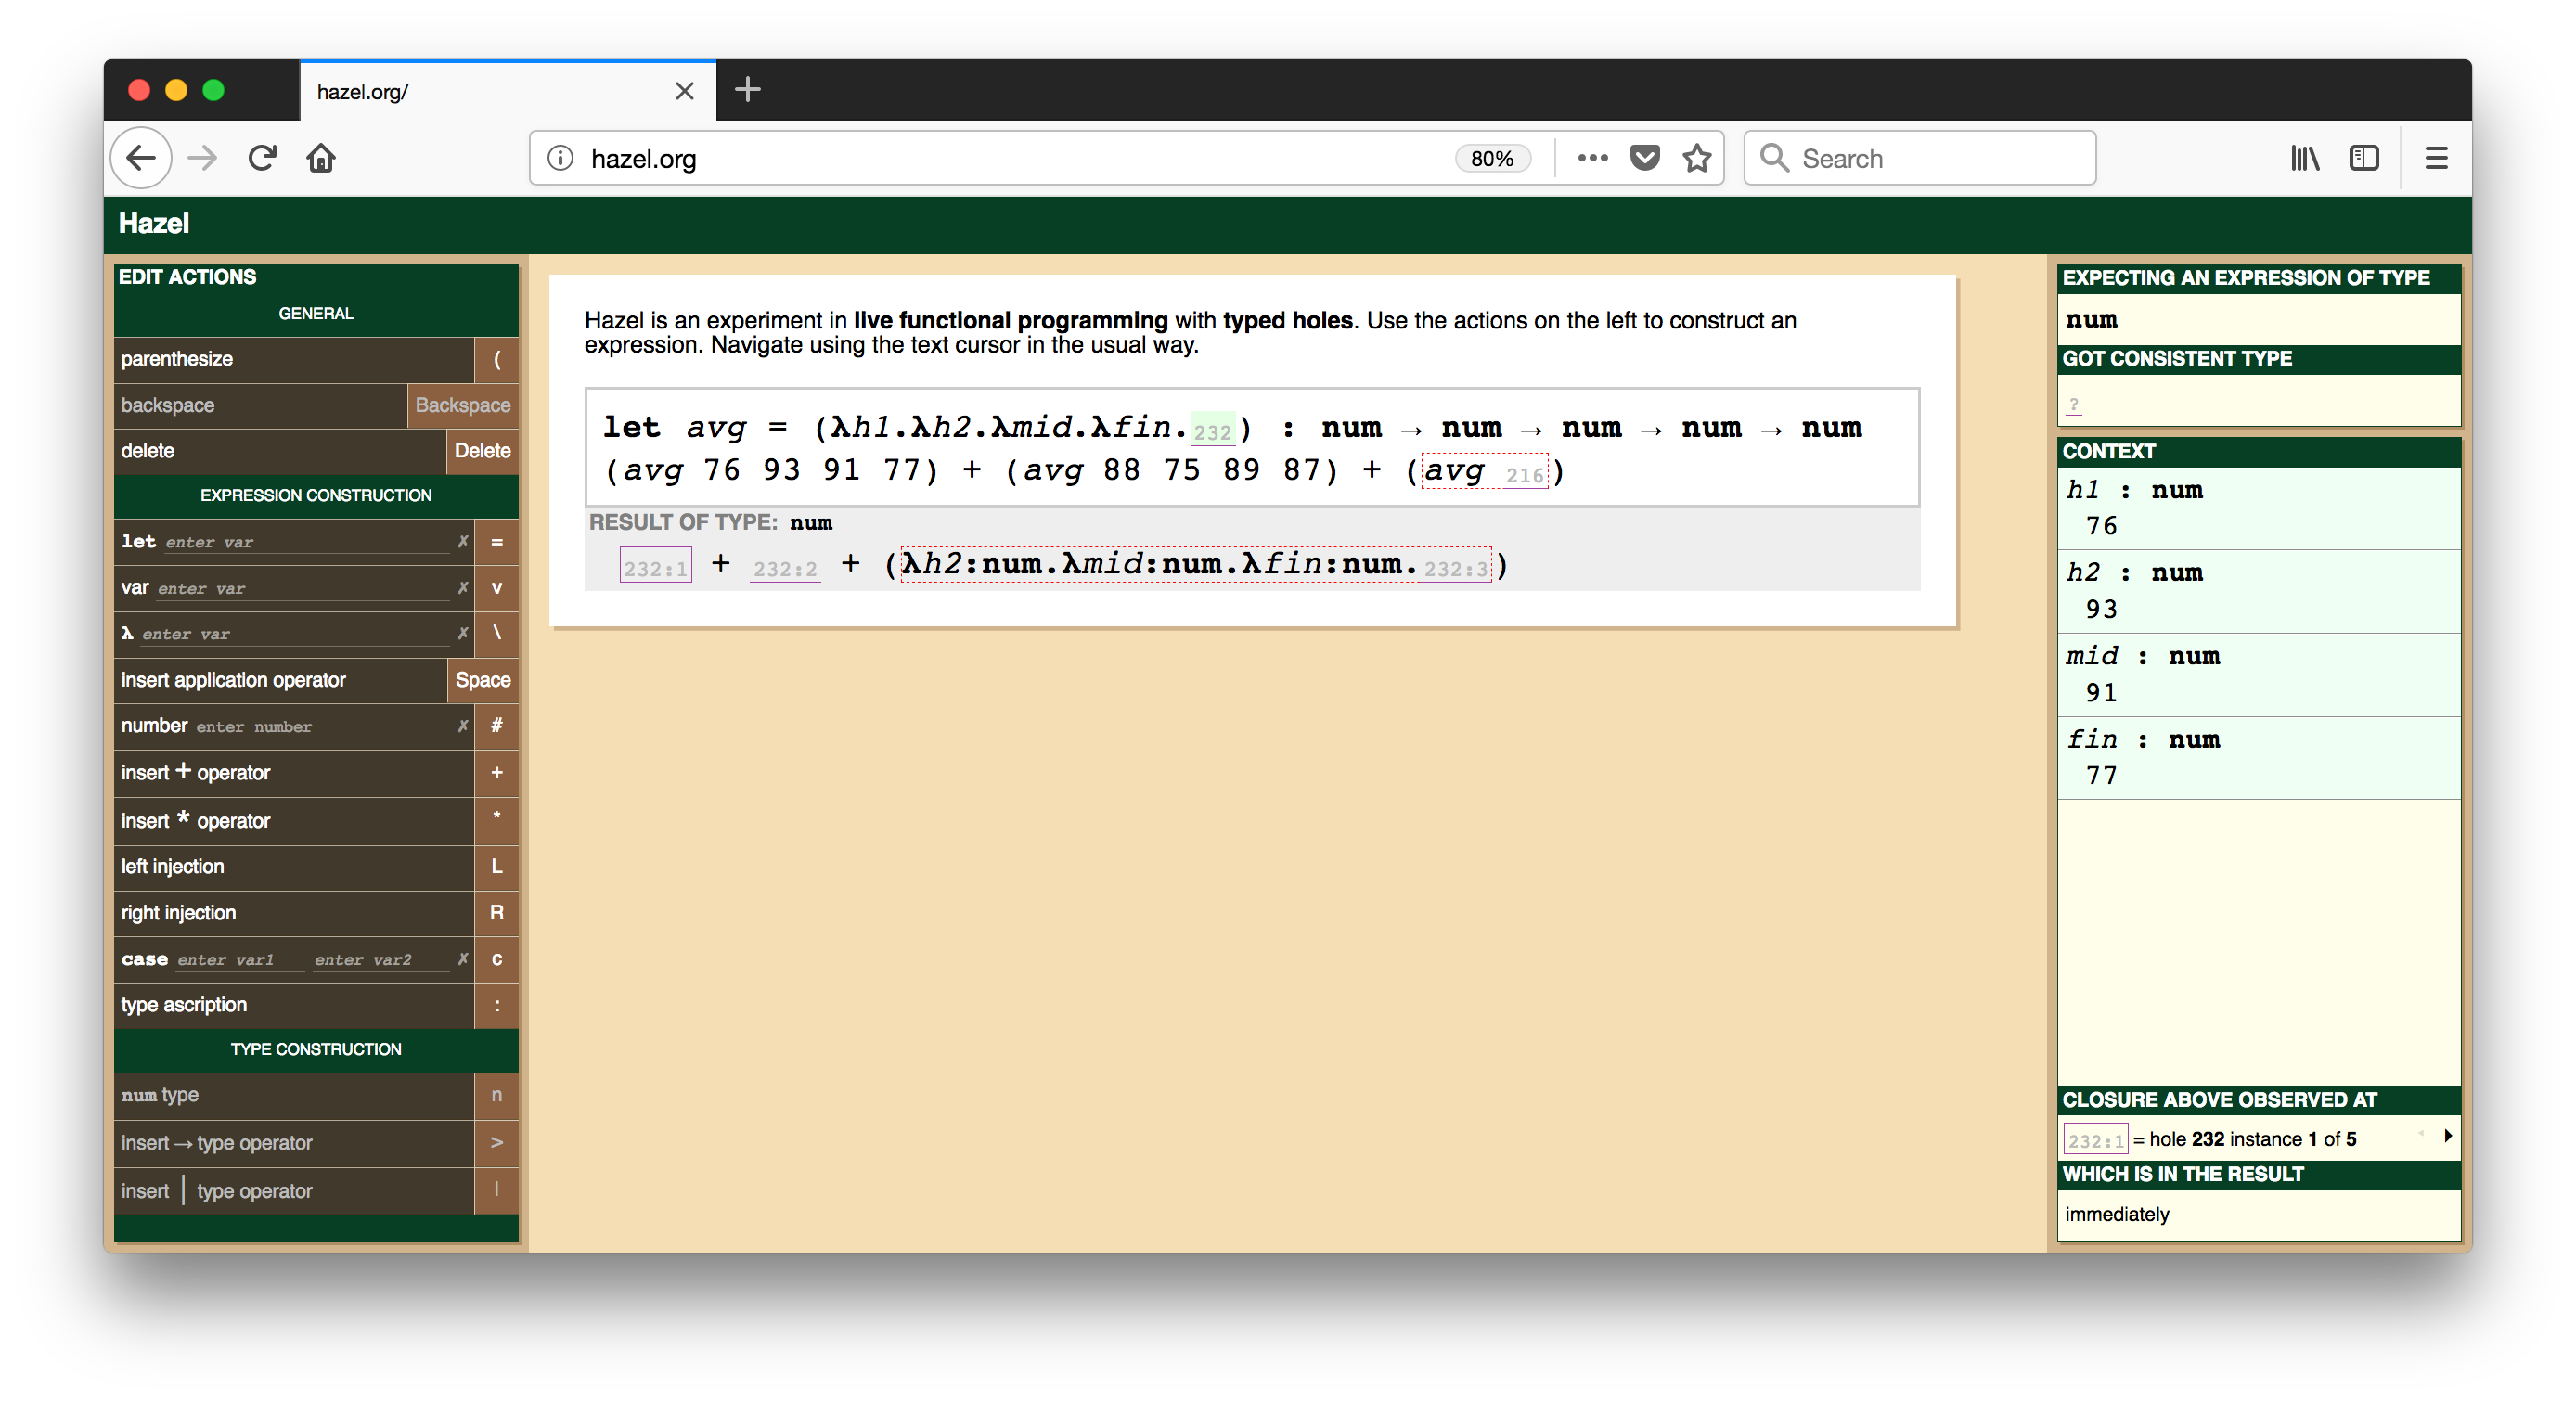
\includegraphics[scale=0.20]{images/hazel-placeholder-0.png}

% \rkc{Draw arrows and captions on the top figure to show how to get
% to the bottom figure.
% ser navigates to hole a, types + to create a plus, types * to create a
% multiplication, types \#10 to create 10, types vh1 to create variable use.}

% 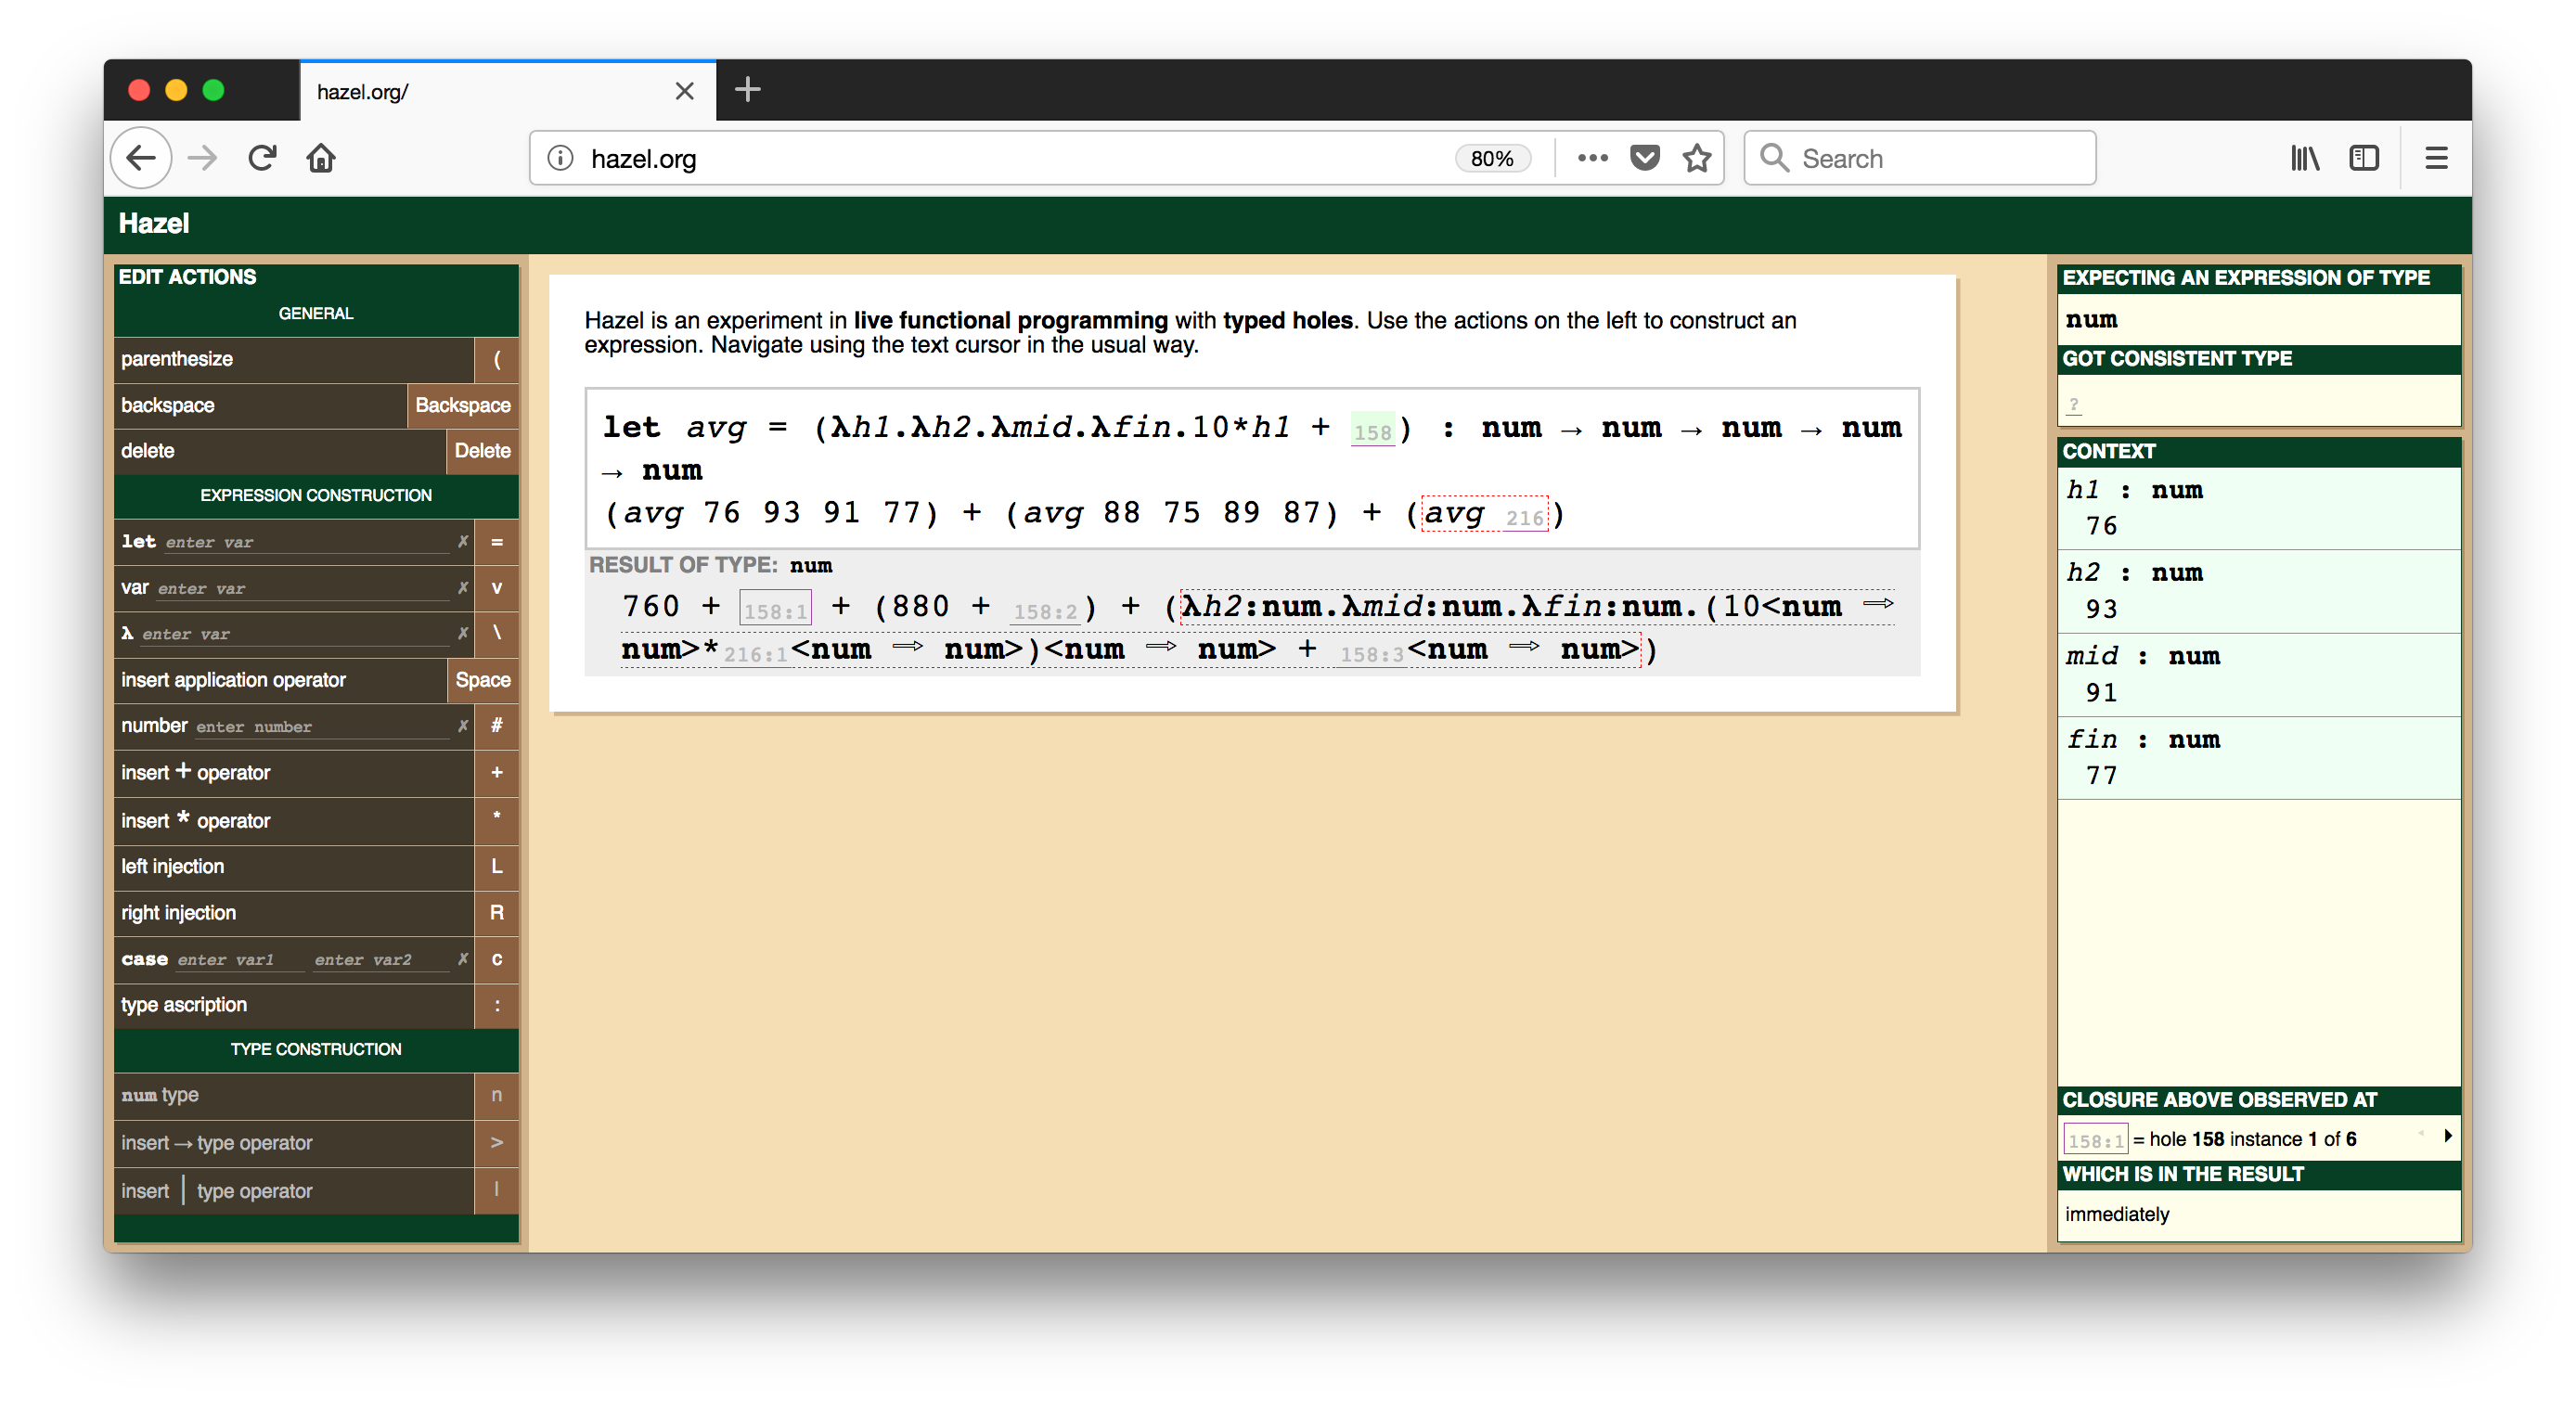
\includegraphics[scale=0.20]{images/hazel-placeholder-1a.png}

\caption{Hazel mockups for Example 1a.}
\label{fig:grades-example}
\end{figure}
